\documentclass[a4paper, 12pt]{article}
\usepackage[top=2cm, bottom=2cm, left=1.5cm, right=1.5cm]{geometry}
\usepackage{graphicx}
\usepackage{float}
\usepackage{pgfplots}


\begin{document}
	\begin{center}
		Universidade Federal do Rio Grande do Norte
		
		Departamento de Engenharia da Computação e Automação
		
		DCA3703 - Programação Paralela
	
		\textbf{Tarefa 2 - Pipeline e vetorização}
		
		\textbf{Aluno:} Daniel Bruno Trindade da Silva
	\end{center}
	
	\section{Introdução}
	Este relatório apresenta os resultados dos estudo realizado para analisar os efeitos de \textbf{Pipeline} e \textbf{Vetorização} em trechos de código em C. O estudo envolveu a implementação e execução de três laços:
	\begin{enumerate}
		\item Inicialização de um vetor com um cálculo simples;
		\item Soma acumulativa sequencial, que cria dependência entre as iterações;
		\item Soma utilizando múltiplas variáveis para quebrar a dependência.
	\end{enumerate}
	As execuções do código foram realizadas com diferentes níveis de otimização do compilador (\texttt{-O0}, \texttt{-O2} e \texttt{-O3}), permitindo avaliar como as técnicas de \emph{loop unrolling}, \emph{vectorização} e reorganização de instruções impactam a performance.
	
	\section{Metodologia}
	Para os testes, foi desenvolvido um programa em C que executa os três laços e mede o tempo de execução utilizando a função \texttt{clock()} convertendo os ticks para segundos. O vetor testado possui \(N = 10^9\) elementos, garantindo que as diferenças de desempenho sejam evidentes dado seu tamanho.
	
	O procedimento adotado foi:
	\begin{itemize}
		\item \textbf{O código:} Implementado como solicitado pela tarefa colocando cada um dos loops em uma função. 
		
		Para o loop de inicialização do array temos:
		\begin{verbatim}
			void init_array(double *array, int size) {
				for (int i = 0; i < size; i++) {
					array[i] = i * 0.3;
				}
			}
		\end{verbatim}
		
		Para o loop com soma acumulativa dependente:
		\begin{verbatim}
			double sum_cumulative(double *array, int size) {
				double sum = 0;
				for (int i = 0; i < size; i++) {
					sum += array[i];
				}
				return sum;
			}
		\end{verbatim}
		
		Para o loop de soma acumulativa de múltiplas variáveis:
		\begin{verbatim}
			double sum_parallel(double *array, int size) {
				double sum1 = 0;
				double sum2 = 0;
				for (int i = 0; i < size; i += 2) {
					sum1 += array[i];
					if (i + 1 < size) {
						sum2 += array[i + 1];
					}
				}
				return sum1 + sum2;
			}
		\end{verbatim}
		
		 
		\item \textbf{Compilação:} O código foi compilado utilizando as diretivas \texttt{-O0}, \texttt{-O2} e \texttt{-O3}:
		\begin{verbatim}
			gcc -O0 tarefa_2.c -o exec_O0
			gcc -O2 tarefa_2.c -o exec_O2
			gcc -O3 tarefa_2.c -o exec_O3
		\end{verbatim}
		\item \textbf{Medição:} Para cada versão compilada, foram registrados os tempos de execução dos laços:
		\begin{itemize}
			\item \textbf{Loop 1:} Inicialização do vetor, sem dependências, que permite uma boa aplicação de vetorização.
			\item \textbf{Loop 2:} Soma acumulativa, onde a dependência entre iterações impede o aproveitamento completo do pipeline.
			\item \textbf{Loop 3:} Soma com múltiplas variáveis, técnica que quebra a dependência e permite otimizações como \emph{loop unrolling}.
		\end{itemize}
		\item \textbf{Análise:} Foram comparados os tempos de execução entre as diferentes diretivas para evidenciar os ganhos de desempenho proporcionados pelas otimizações.
	\end{itemize}
	
	\section{Resultados e Discussão}
	
	Como resultado obtivemos o tempo de execução para cada laço e como esse tempo muda a medida que trocamos o nível de otimização utilizada para compilar. Na figura a baixo podemos ver o retorno do código:
	
	\begin{figure}[h]
		\centering
		\includegraphics[width=0.79\textwidth]{resultados.png}
		\caption{Resultados da execução do código com níveis diferentes de otimização}
		\label{figura:exemplo}
	\end{figure}
	
	A seguir organizamos os resultados obtidos em uma tabela com os níveis de otimização nas colunas e os loops trabalhados nas linhas facilitando assim a análise:
	
	\begin{table}[H]
		\centering
		\begin{tabular}{|c|c|c|c|}
			\hline
			\textbf{} & \textbf{-O0} & \textbf{-O2} & \textbf{-O3} \\
			\hline
			Loop 1 & 3.731660s & 2.227655s & 1.958283s \\
			\hline
			Loop 2 & 2.256485s & 1.023743s & 1.016616s \\
			\hline
			Loop 3 & 1.325182s & 0.625898s & 0.602650s \\
			\hline
		\end{tabular}
		\caption{Tempo de execução (em segundos) para diferentes níveis de otimização}
		\label{tab:resultados}
	\end{table}
	
	Se considerarmos o o0 como ponto de partida para sabermos o ganho de tempo que temos em cada otimização teremos o seguinte gráfico:
	
	\begin{figure}[h!]
		\centering
		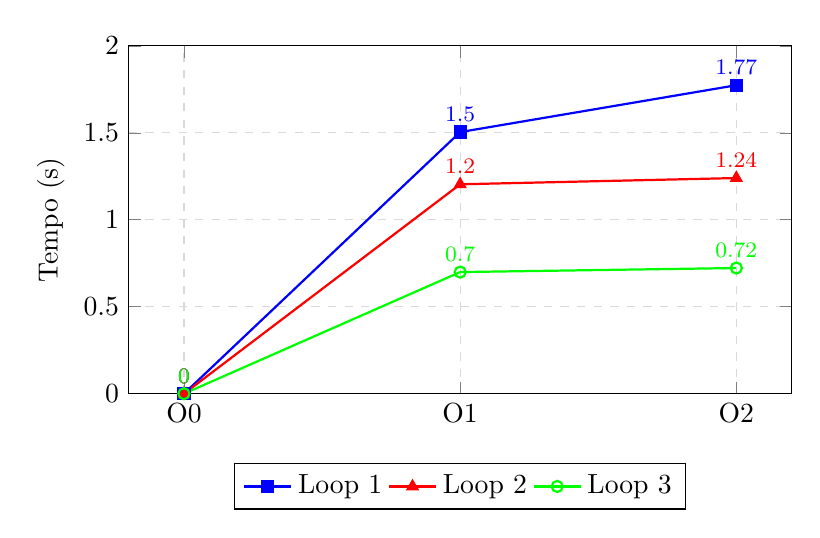
\begin{tikzpicture}
			\begin{axis}[
				width=10cm, height=6cm,
				xlabel={Nível de Otimização},
				xlabel style={yshift=-10pt},
				ylabel={Tempo (s)},
				grid=both,
				grid style={dashed, gray!30},
				legend style={at={(0.5,-0.2)}, anchor=north, legend columns=3},
				ymin=0, ymax=2,
				symbolic x coords={O0, O1, O2},
				xtick=data,
				nodes near coords,
				every node near coord/.append style={font=\footnotesize}, % Define o tamanho da fonte
				]
				
				% Tempo de execução Loop 1 (Azul)
				\addplot[
				color=blue,
				mark=square*,
				thick,
				] coordinates {
					(O0, 0)
					(O1, 1.504005)
					(O2, 1.773377)
				};
				\addlegendentry{Loop 1}
				
				% Tempo de execução Loop 2 (Vermelho)
				\addplot[
				color=red,
				mark=triangle*,
				thick,
				] coordinates {
					(O0, 0)
					(O1, 1.203912)
					(O2, 1.239869)
				};
				\addlegendentry{Loop 2}
				
				% Tempo de execução Loop 3 (Verde)
				\addplot[
				color=green,
				mark=o,
				thick,
				] coordinates {
					(O0, 0)
					(O1, 0.699284)
					(O2, 0.722532)
				};
				\addlegendentry{Loop 3}
				
			\end{axis}
		\end{tikzpicture}
		\caption{Comparação do Tempo de Execução por Nível de Otimização}
	\end{figure}

	
	
	Analisando os resultados dos loops individualmente a medida que aplicamos as otimizações, podemos observar que:	
	
	\begin{itemize}
		\item \textbf{Loop 1:} Apresenta o melhor ganho de desempenho ao aplicarmos as otimizações. Isso se deve ao fato de que o loop 1 é um candidato ideal para vetorização, porque ele tem operações simples e previsíveis, não há dependências entre iterações e a CPU pode carregar e armazenar múltiplos valores simultaneamente usando registradores vetoriais;
		
		\item \textbf{Loop 2:} O desempenho é inferior devido à soma sequencial, em que cada iteração depende da anterior, limitando assim as otimizações, por exemplo o Loop 2 requer mais acessos simultâneos à memória, o que pode causar mais "cache misses" (falhas na cache), aumentando a latência. Além disso, como estamos somando valores ao próprio vetor, o processador precisa esperar o valor anterior estar carregado antes de prosseguir, limitando a otimização. Ainda assim ele tem um certo ganho de desempenho com as otimizações pois o compilador consegue aplicar parcialmente a vetorização fazendo com que algumas operações possam ser realizadas em paralelo;
		
		\item \textbf{Loop 3:} Teve o menor ganho de desempenho em relação aos outros loops quando aumentamos o nível de otimização porque o Loop 3 já reduz dependências de dados em seu código. Esse loop utiliza duas variáveis (sum1 e sum2) para acumular valores de elementos intercalados do array. Isso reduz a dependência entre iterações consecutivas do laço, permitindo que o compilador já aproveite paralelismo e vetorização, mesmo sem otimizações agressivas. Ou seja, o Loop 3 já nasce otimizado. Com isso, os ganhos adicionais das otimizações -O1 e -O2 são limitados.
	\end{itemize}
	
	As diretivas de compilação influenciam fortemente esses resultados pois são elas que controlam o nível de otimização que será aplicada da seguinte forma:
	
	\begin{itemize}
		\item \texttt{-O0} não aplica otimizações, resultando em execução mais lenta e nas operações ocorrendo na ordem exata do código.
		\item \texttt{-O2} já emprega otimizações moderadas, como vetorização e inlining, melhorando o desempenho dos laços sem dependências.
		\item \texttt{-O3} utiliza otimizações agressivas, maximizando o ganho de performance, principalmente em laços que permitem reordenação das instruções.
	\end{itemize}
	
	\section{Conclusão}
	Os experimentos realizados evidenciam a importância de se estruturar o código de forma a favorecer a extração de paralelismo a nível de instrução (ILP). A quebra de dependência, conforme demonstrado no Loop 1, permite que o compilador aplique técnicas avançadas de otimização, resultando em ganhos expressivos de desempenho. Este estudo reforça a relevância das otimizações de \emph{pipeline} e \emph{vetorização} no desenvolvimento de aplicações em computação paralela.
	
	
	
	
	
\end{document}